\section*{Simulated Total Energy vs. Time (varying COR)}

% sim-001 total energy
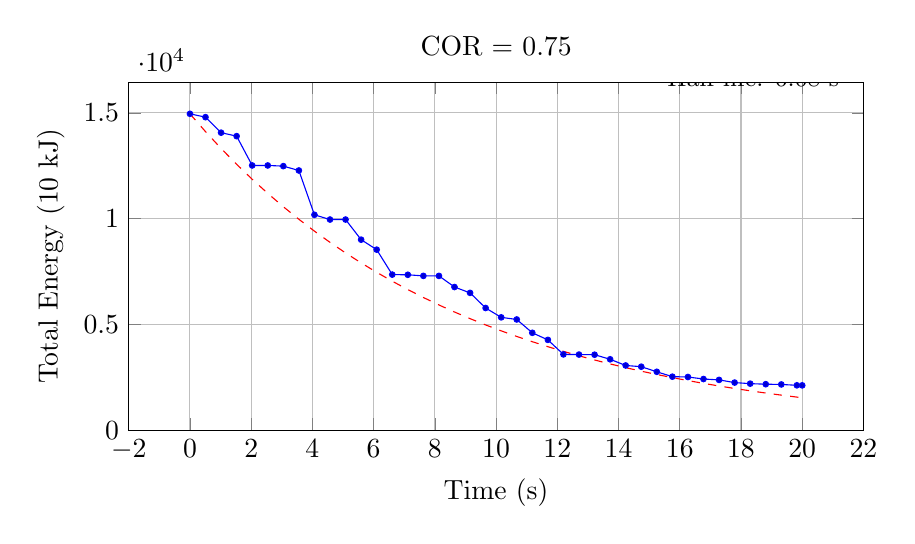
\begin{tikzpicture}
\begin{axis}[
    width=0.9\textwidth,
    height=6cm,
    xlabel={Time (s)},
    ylabel={Total Energy (10 kJ)},
    title={COR = 0.75},
    grid=both,
    tick label style={/pgf/number format/fixed},
    ymin=0,
]
\addplot+[mark=*, mark size=1pt] coordinates {
(0.0,14952.35)
(0.5083333313000006,14793.449377865778)
(1.0166666625999987,14060.99750925699)
(1.5249999938999967,13896.477440682682)
(2.0333333251999948,12510.882701954857)
(2.541666656499993,12510.88270195486)
(3.049999987799991,12479.417453684833)
(3.558333319099989,12273.363378570186)
(4.06666665039999,10177.437401698673)
(4.5749999817000155,9953.755916310372)
(5.083333313000041,9953.755916310378)
(5.591666644300066,9002.041334518524)
(6.099999975600091,8530.583665838883)
(6.608333306900116,7350.988837906317)
(7.116666638200141,7342.441980877146)
(7.624999969500166,7290.264841132356)
(8.133333300800178,7290.264841132361)
(8.641666632100149,6763.498647989738)
(9.14999996340012,6487.124076635238)
(9.65833329470009,5772.572317610013)
(10.166666626000062,5329.722018976285)
(10.674999957300033,5230.0151650428525)
(11.183333288600004,4599.122403695114)
(11.691666619899975,4264.852754860962)
(12.199999951199946,3578.1682360247087)
(12.708333282499916,3570.672635253077)
(13.216666613799887,3564.085241381409)
(13.724999945099858,3347.1138177804833)
(14.23333327639983,3054.998878267983)
(14.7416666076998,2997.0310074787008)
(15.249999938999771,2756.1710588494307)
(15.758333270299742,2526.3793017135954)
(16.26666660159977,2510.3000125844205)
(16.77499993289985,2414.674124740351)
(17.28333326419993,2373.3887490235866)
(17.791666595500008,2245.9090397318696)
(18.299999926800087,2195.9169572877395)
(18.808333258100166,2169.7127961186698)
(19.316666589400246,2157.634562192314)
(19.824999920700325,2117.2402358938666)
(19.999999920000352,2114.986428980833)
};
\addplot+[red,dashed,mark=none] coordinates {
(0.0,14952.35)
(0.5083333313000006,14110.489801679527)
(1.0166666625999987,13316.02874754149)
(1.5249999938999967,12566.29812979603)
(2.0333333251999948,11858.779496557492)
(2.541666656499993,11191.096192005994)
(3.049999987799991,10561.005372862139)
(3.558333319099989,9966.39047435714)
(4.06666665039999,9405.254100390399)
(4.5749999817000155,8875.711313991642)
(5.083333313000041,8375.983305549313)
(5.591666644300066,7904.391417535789)
(6.099999975600091,7459.351505657745)
(6.608333306900116,7039.36861748997)
(7.116666638200141,6643.031970717302)
(7.624999969500166,6269.010214115994)
(8.133333300800178,5916.046955355406)
(8.641666632100149,5582.956540597294)
(9.14999996340012,5268.620071715711)
(9.65833329470009,4971.98164775897)
(10.166666626000062,4692.044818028)
(10.674999957300033,4427.869234856566)
(11.183333288600004,4178.5674948495935)
(11.691666619899975,3943.3021579688116)
(12.199999951199946,3721.282934452442)
(12.708333282499916,3511.764030119374)
(13.216666613799887,3314.0416411403285)
(13.724999945099858,3127.451589860594)
(14.23333327639983,2951.3670937327233)
(14.7416666076998,2785.1966598647223)
(15.249999938999771,2628.3820981112117)
(15.758333270299742,2480.39664603326)
(16.26666660159977,2340.743199428338)
(16.77499993289985,2208.952642486564)
(17.28333326419993,2084.5822719639004)
(17.791666595500008,1967.2143100789028)
(18.299999926800087,1856.45450113769)
(18.808333258100166,1751.9307871729325)
(19.316666589400246,1653.2920581481728)
(19.824999920700325,1560.206972529223)
(19.999999920000352,1529.389272231035)
};
\node[anchor=south east, font=\small] at (rel axis cs:0.98,0.96) {Half-life: 6.08 s};
\end{axis}
\end{tikzpicture}


% sim-002 total energy
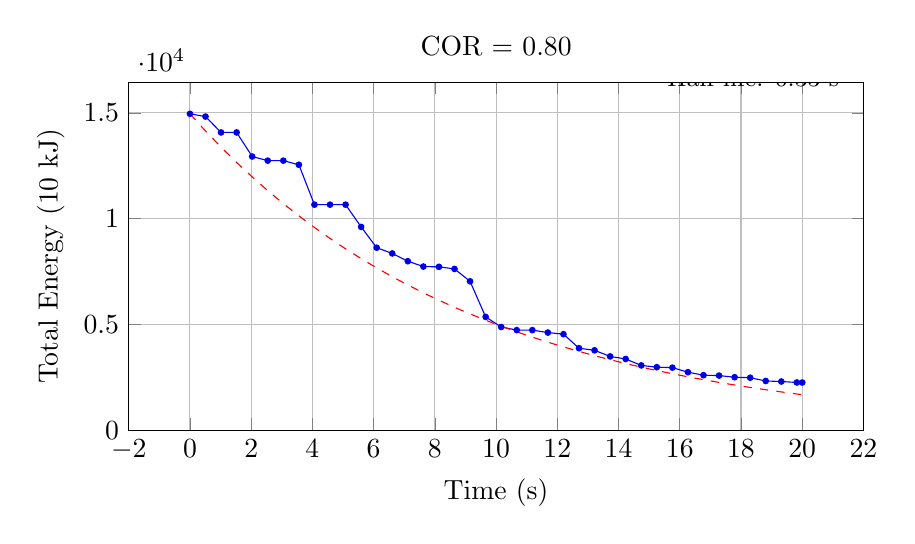
\begin{tikzpicture}
\begin{axis}[
    width=0.9\textwidth,
    height=6cm,
    xlabel={Time (s)},
    ylabel={Total Energy (10 kJ)},
    title={COR = 0.80},
    grid=both,
    tick label style={/pgf/number format/fixed},
    ymin=0,
]
\addplot+[mark=*, mark size=1pt] coordinates {
(0.0,14952.35)
(0.5083333313000006,14821.69007714793)
(1.0166666625999987,14071.647349413635)
(1.5249999938999967,14071.647349413639)
(2.0333333251999948,12934.244846683321)
(2.541666656499993,12738.379122106688)
(3.049999987799991,12738.379122106693)
(3.558333319099989,12543.228484878187)
(4.06666665039999,10658.38604491867)
(4.5749999817000155,10658.386044918667)
(5.083333313000041,10658.386044918669)
(5.591666644300066,9605.809429482122)
(6.099999975600091,8623.339413409078)
(6.608333306900116,8351.50728562189)
(7.116666638200141,7984.009455230087)
(7.624999969500166,7731.31373067596)
(8.133333300800178,7718.229943083752)
(8.641666632100149,7619.9053856341325)
(9.14999996340012,7033.329538183809)
(9.65833329470009,5352.004190407549)
(10.166666626000062,4873.502175461628)
(10.674999957300033,4726.972847669426)
(11.183333288600004,4725.859533409453)
(11.691666619899975,4610.8075076882615)
(12.199999951199946,4534.565748084708)
(12.708333282499916,3871.624178330014)
(13.216666613799887,3771.282518514108)
(13.724999945099858,3482.468425705953)
(14.23333327639983,3361.8662908606675)
(14.7416666076998,3057.949471982987)
(15.249999938999771,2973.928964419454)
(15.758333270299742,2953.5395957848323)
(16.26666660159977,2738.0024987456713)
(16.77499993289985,2594.9732927669647)
(17.28333326419993,2576.14073308934)
(17.791666595500008,2499.6341183852155)
(18.299999926800087,2476.2558583775617)
(18.808333258100166,2321.2826192069074)
(19.316666589400246,2296.6136211563776)
(19.824999920700325,2251.026132346474)
(19.999999920000352,2247.8934615111625)
};
\addplot+[red,dashed,mark=none] coordinates {
(0.0,14952.35)
(0.5083333313000006,14142.948278717964)
(1.0166666625999987,13377.361151557545)
(1.5249999938999967,12653.216843653967)
(2.0333333251999948,11968.271969235677)
(2.541666656499993,11320.404581656408)
(3.049999987799991,10707.607599643434)
(3.558333319099989,10127.982589396619)
(4.06666665039999,9579.733883275365)
(4.5749999817000155,9061.16301685321)
(5.083333313000041,8570.663467106284)
(5.591666644300066,8106.7156754343905)
(6.099999975600091,7667.882340096403)
(6.608333306900116,7252.803963475842)
(7.116666638200141,6860.194640382228)
(7.624999969500166,6488.838074340405)
(8.133333300800178,6137.583809526403)
(8.641666632100149,5805.343666676406)
(9.14999996340012,5491.088371927327)
(9.65833329470009,5193.844368145346)
(10.166666626000062,4912.690798863754)
(10.674999957300033,4646.756655486524)
(11.183333288600004,4395.218078919674)
(11.691666619899975,4157.295807270916)
(12.199999951199946,3932.252761710621)
(12.708333282499916,3719.3917630151354)
(13.216666613799887,3518.0533717183484)
(13.724999945099858,3327.613845180331)
(14.23333327639983,3147.483205244084)
(14.7416666076998,2977.103410494047)
(15.249999938999771,2815.946627454032)
(15.758333270299742,2663.5135953688073)
(16.26666660159977,2519.332079503426)
(16.77499993289985,2382.955408168724)
(17.28333326419993,2253.9610889406163)
(17.791666595500008,2131.9494997863)
(18.299999926800087,2016.5426510425461)
(18.808333258100166,1907.383014410664)
(19.316666589400246,1804.1324153403946)
(19.824999920700325,1706.4709853713623)
(19.999999920000352,1674.0879121003832)
};
\node[anchor=south east, font=\small] at (rel axis cs:0.98,0.96) {Half-life: 6.33 s};
\end{axis}
\end{tikzpicture}


% sim-003 total energy
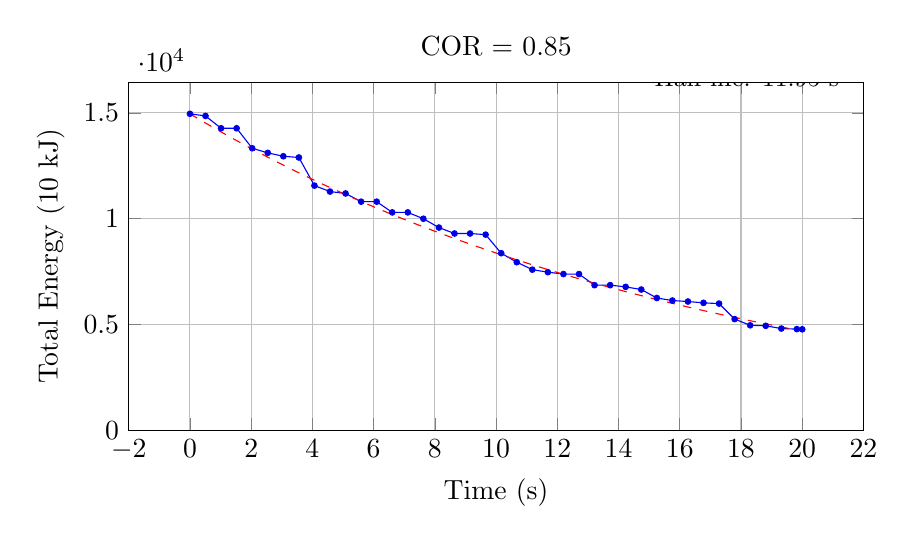
\begin{tikzpicture}
\begin{axis}[
    width=0.9\textwidth,
    height=6cm,
    xlabel={Time (s)},
    ylabel={Total Energy (10 kJ)},
    title={COR = 0.85},
    grid=both,
    tick label style={/pgf/number format/fixed},
    ymin=0,
]
\addplot+[mark=*, mark size=1pt] coordinates {
(0.0,14952.35)
(0.5083333313000006,14851.752757028931)
(1.0166666625999987,14269.774127311952)
(1.5249999938999967,14269.774127311957)
(2.0333333251999948,13324.09087755664)
(2.541666656499993,13105.777090489755)
(3.049999987799991,12945.833592323303)
(3.558333319099989,12887.07269580071)
(4.06666665039999,11558.32581884131)
(4.5749999817000155,11276.214354634007)
(5.083333313000041,11187.020904263554)
(5.591666644300066,10799.783953241065)
(6.099999975600091,10799.783953241067)
(6.608333306900116,10291.540733043772)
(7.116666638200141,10291.540733043774)
(7.624999969500166,9992.097843827984)
(8.133333300800178,9574.687556423729)
(8.641666632100149,9293.931012948942)
(9.14999996340012,9293.931012948946)
(9.65833329470009,9240.14829450998)
(10.166666626000062,8363.266171947203)
(10.674999957300033,7938.199364991653)
(11.183333288600004,7584.849294897862)
(11.691666619899975,7465.314625225458)
(12.199999951199946,7376.622078878891)
(12.708333282499916,7376.622078878893)
(13.216666613799887,6852.383960030509)
(13.724999945099858,6852.383960030509)
(14.23333327639983,6770.419131491028)
(14.7416666076998,6645.620708364326)
(15.249999938999771,6245.550147907972)
(15.758333270299742,6124.800404880835)
(16.26666660159977,6078.160465102783)
(16.77499993289985,6014.876037743097)
(17.28333326419993,5980.574755501706)
(17.791666595500008,5247.79596518493)
(18.299999926800087,4954.183959951206)
(18.808333258100166,4929.9300151061025)
(19.316666589400246,4801.025100072453)
(19.824999920700325,4774.244710367897)
(19.999999920000352,4765.0503661848115)
};
\addplot+[red,dashed,mark=none] coordinates {
(0.0,14952.35)
(0.5083333313000006,14517.792675356724)
(1.0166666625999987,14095.86480818342)
(1.5249999938999967,13686.199350942421)
(2.0333333251999948,13288.439923529335)
(2.541666656499993,12902.240503247453)
(3.049999987799991,12527.265123792364)
(3.558333319099989,12163.18758298492)
(4.06666665039999,11809.691158998305)
(4.5749999817000155,11466.468334832343)
(5.083333313000041,11133.2205307954)
(5.591666644300066,10809.657844761012)
(6.099999975600091,10495.498799973484)
(6.608333306900116,10190.470100182922)
(7.116666638200141,9894.306391896735)
(7.624999969500166,9606.750033540773)
(8.133333300800178,9327.550871329331)
(8.641666632100149,9056.466021648932)
(9.14999996340012,8793.259659766669)
(9.65833329470009,8537.702814679333)
(10.166666626000062,8289.573169924748)
(10.674999957300033,8048.654870182101)
(11.183333288600004,7814.738333493004)
(11.691666619899975,7587.620068939955)
(12.199999951199946,7367.102499623561)
(12.708333282499916,7152.993790784548)
(13.216666613799887,6945.107682921026)
(13.724999945099858,6743.263329755841)
(14.23333327639983,6547.285140913042)
(14.7416666076998,6357.002629166615)
(15.249999938999771,6172.250262128607)
(15.758333270299742,5992.867318247597)
(16.26666660159977,5818.697746992247)
(16.77499993289985,5649.590033098364)
(17.28333326419993,5485.397064761284)
(17.791666595500008,5325.976005658929)
(18.299999926800087,5171.188170694273)
(18.808333258100166,5020.8989053490795)
(19.316666589400246,4874.97746854395)
(19.824999920700325,4733.296918902788)
(19.999999920000352,4685.48055136778)
};
\node[anchor=south east, font=\small] at (rel axis cs:0.98,0.96) {Half-life: 11.95 s};
\end{axis}
\end{tikzpicture}


% sim-004 total energy
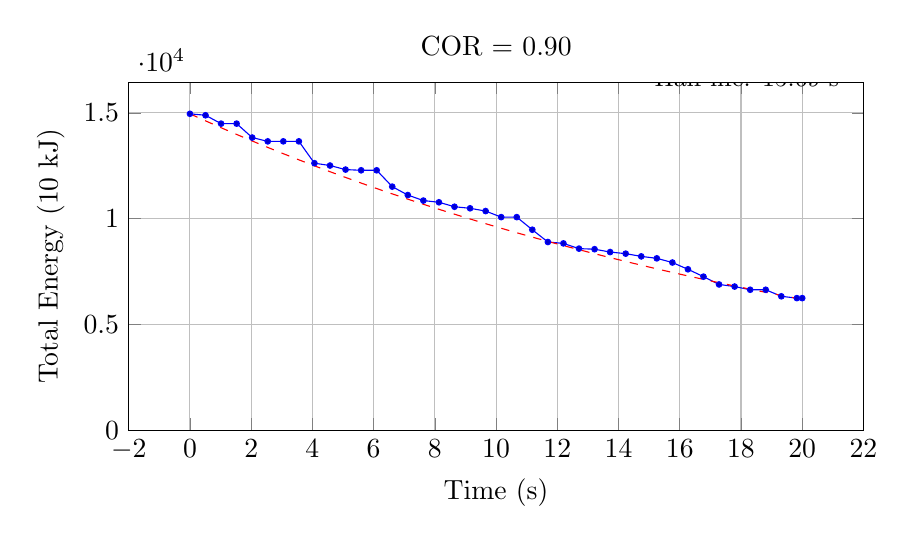
\begin{tikzpicture}
\begin{axis}[
    width=0.9\textwidth,
    height=6cm,
    xlabel={Time (s)},
    ylabel={Total Energy (10 kJ)},
    title={COR = 0.90},
    grid=both,
    tick label style={/pgf/number format/fixed},
    ymin=0,
]
\addplot+[mark=*, mark size=1pt] coordinates {
(0.0,14952.35)
(0.5083333313000006,14883.637417508777)
(1.0166666625999987,14488.391569414702)
(1.5249999938999967,14488.391569414707)
(2.0333333251999948,13829.669651831377)
(2.541666656499993,13650.30903544757)
(3.049999987799991,13650.309035447572)
(3.558333319099989,13650.309035447579)
(4.06666665039999,12617.675594326334)
(4.5749999817000155,12506.993280713672)
(5.083333313000041,12315.57246875409)
(5.591666644300066,12282.231860066082)
(6.099999975600091,12282.231860066086)
(6.608333306900116,11509.505184735082)
(7.116666638200141,11111.630001406054)
(7.624999969500166,10850.701433943392)
(8.133333300800178,10770.007503233082)
(8.641666632100149,10559.056507093683)
(9.14999996340012,10485.739489145748)
(9.65833329470009,10355.050610290382)
(10.166666626000062,10068.334431774927)
(10.674999957300033,10068.334431774938)
(11.183333288600004,9472.32074139948)
(11.691666619899975,8891.811344193096)
(12.199999951199946,8826.64482766262)
(12.708333282499916,8578.738336519204)
(13.216666613799887,8552.015175675047)
(13.724999945099858,8416.75900832302)
(14.23333327639983,8341.365578060699)
(14.7416666076998,8212.060450930816)
(15.249999938999771,8119.604128347984)
(15.758333270299742,7922.127945247138)
(16.26666660159977,7601.79178488001)
(16.77499993289985,7253.939646604871)
(17.28333326419993,6885.187327559558)
(17.791666595500008,6785.7942797142405)
(18.299999926800087,6634.20852235607)
(18.808333258100166,6634.208522356072)
(19.316666589400246,6324.424683354282)
(19.824999920700325,6238.8247721669595)
(19.999999920000352,6238.8247721669595)
};
\addplot+[red,dashed,mark=none] coordinates {
(0.0,14952.35)
(0.5083333313000006,14620.290315446524)
(1.0166666625999987,14295.604965636803)
(1.5249999938999967,13978.130182382638)
(2.0333333251999948,13667.705834436707)
(2.541666656499993,13364.17534672389)
(3.049999987799991,13067.385621366308)
(3.558333319099989,12777.186960462204)
(4.06666665039999,12493.432990579753)
(4.5749999817000155,12215.9805889277)
(5.083333313000041,11944.689811165614)
(5.591666644300066,11679.423820817277)
(6.099999975600091,11420.048820251674)
(6.608333306900116,11166.433983196746)
(7.116666638200141,10918.45138875188)
(7.624999969500166,10675.975956865817)
(8.133333300800178,10438.88538524748)
(8.641666632100149,10207.060087677872)
(9.14999996340012,9980.383133691876)
(9.65833329470009,9758.740189599719)
(10.166666626000062,9542.019460818115)
(10.674999957300033,9330.111635482152)
(11.183333288600004,9122.909829309428)
(11.691666619899975,8920.309531688643)
(12.199999951199946,8722.208552965454)
(12.708333282499916,8528.506972898964)
(13.216666613799887,8339.107090262938)
(13.724999945099858,8153.913373566219)
(14.23333327639983,7972.832412867559)
(14.7416666076998,7795.772872660543)
(15.249999938999771,7622.645445804828)
(15.758333270299742,7453.362808480474)
(16.26666660159977,7287.839576142631)
(16.77499993289985,7125.992260454419)
(17.28333326419993,6967.7392271762155)
(17.791666595500008,6813.000654990079)
(18.299999926800087,6661.698495238671)
(18.808333258100166,6513.756432558246)
(19.316666589400246,6369.09984638592)
(19.824999920700325,6227.655773321764)
(19.999999920000352,6179.692306595814)
};
\node[anchor=south east, font=\small] at (rel axis cs:0.98,0.96) {Half-life: 15.69 s};
\end{axis}
\end{tikzpicture}


% sim-005 total energy
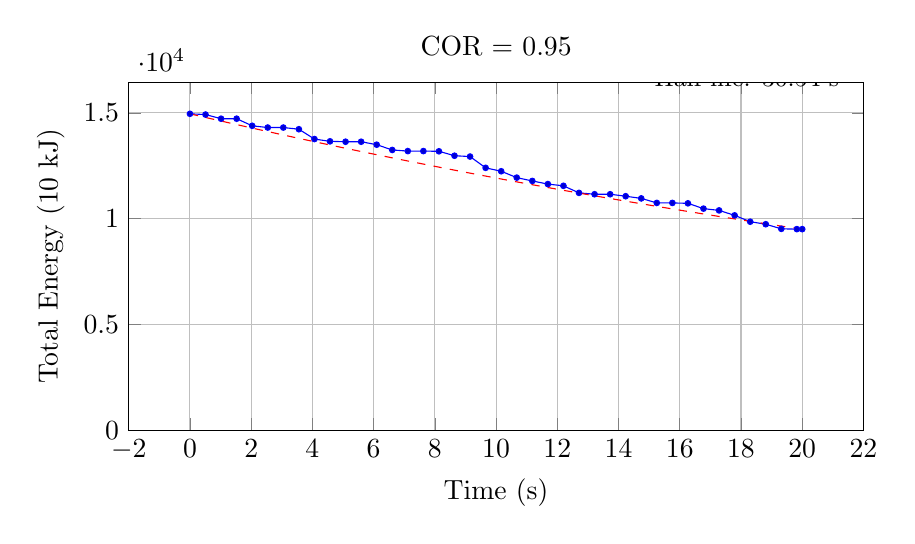
\begin{tikzpicture}
\begin{axis}[
    width=0.9\textwidth,
    height=6cm,
    xlabel={Time (s)},
    ylabel={Total Energy (10 kJ)},
    title={COR = 0.95},
    grid=both,
    tick label style={/pgf/number format/fixed},
    ymin=0,
]
\addplot+[mark=*, mark size=1pt] coordinates {
(0.0,14952.35)
(0.5083333313000006,14917.344058587474)
(1.0166666625999987,14721.297834707682)
(1.5249999938999967,14721.297834707688)
(2.0333333251999948,14385.709382792906)
(2.541666656499993,14303.327247480476)
(3.049999987799991,14303.327247480478)
(3.558333319099989,14224.456354241931)
(4.06666665039999,13758.78596468365)
(4.5749999817000155,13651.011602345641)
(5.083333313000041,13632.873725656009)
(5.591666644300066,13632.873725656007)
(6.099999975600091,13492.80977177181)
(6.608333306900116,13243.516785691252)
(7.116666638200141,13190.430226717777)
(7.624999969500166,13190.430226717774)
(8.133333300800178,13179.932187211783)
(8.641666632100149,12971.439398971932)
(9.14999996340012,12931.391408916594)
(9.65833329470009,12398.047163211495)
(10.166666626000062,12237.073166969152)
(10.674999957300033,11935.032861552918)
(11.183333288600004,11778.632063766778)
(11.691666619899975,11630.79688501585)
(12.199999951199946,11548.41113239637)
(12.708333282499916,11214.734162165641)
(13.216666613799887,11150.200307127694)
(13.724999945099858,11150.200307127694)
(14.23333327639983,11056.409146557951)
(14.7416666076998,10953.76940471673)
(15.249999938999771,10739.834609102109)
(15.758333270299742,10739.834609102109)
(16.26666660159977,10720.409006952661)
(16.77499993289985,10470.105717219214)
(17.28333326419993,10386.287274176468)
(17.791666595500008,10151.675723029626)
(18.299999926800087,9852.237392217707)
(18.808333258100166,9732.927374766652)
(19.316666589400246,9514.565840541203)
(19.824999920700325,9500.540144051993)
(19.999999920000352,9500.540144051993)
};
\addplot+[red,dashed,mark=none] coordinates {
(0.0,14952.35)
(0.5083333313000006,14780.803994427997)
(1.0166666625999987,14611.22610972179)
(1.5249999938999967,14443.593765934218)
(2.0333333251999948,14277.884642174362)
(2.541666656499993,14114.076673635445)
(3.049999987799991,13952.14804865682)
(3.558333319099989,13792.077205819654)
(4.06666665039999,13633.842831075948)
(4.5749999817000155,13477.423854910485)
(5.083333313000041,13322.799449535352)
(5.591666644300066,13169.949026116641)
(6.099999975600091,13018.852232032947)
(6.608333306900116,12869.488948165359)
(7.116666638200141,12721.839286218512)
(7.624999969500166,12575.883586072388)
(8.133333300800178,12431.602413164499)
(8.641666632100149,12288.976555902093)
(9.14999996340012,12147.987023104046)
(9.65833329470009,12008.615041472136)
(10.166666626000062,11870.842053091292)
(10.674999957300033,11734.649712958546)
(11.183333288600004,11600.019886540318)
(11.691666619899975,11466.934647357735)
(12.199999951199946,11335.376274599652)
(12.708333282499916,11205.327250763057)
(13.216666613799887,11076.770259320547)
(13.724999945099858,10949.688182414571)
(14.23333327639983,10824.06409857811)
(14.7416666076998,10699.881280481537)
(15.249999938999771,10577.12319270529)
(15.758333270299742,10455.773489538129)
(16.26666660159977,10335.816012800628)
(16.77499993289985,10217.234789693666)
(17.28333326419993,10100.014030671604)
(17.791666595500008,9984.138127339807)
(18.299999926800087,9869.591650376351)
(18.808333258100166,9756.359347477533)
(19.316666589400246,9644.426141326989)
(19.824999920700325,9533.77712758807)
(19.999999920000352,9495.979323694375)
};
\node[anchor=south east, font=\small] at (rel axis cs:0.98,0.96) {Half-life: 30.54 s};
\end{axis}
\end{tikzpicture}
